\subsection{Painel do docente}

Nesta secção serão referidas todas as soluções já implementadas para o painel do docente.

Serão demonstradas todas as páginas e funcionalidades já implementadas para este tipo de utilizadores, com justificações para as decisões tomadas.

Um dos aspetos que se teve em atenção, no desenvolvimento do painel do docente foi a semelhança em relação ao painel do aluno. Ao haver uma semelhança entre os dois painéis, evita-se que o docente tenha a preocupação de verificar que a informação contida disponível é facilmente acedida pelos alunos.

Em todas as páginas, o docente terá acesso a um cabeçalho onde poderá voltar à página inicial, ao carregar no logótipo, ou terminar a sua sessão no botão mais à direita.

Para além do referido cabeçalho o docente terá acesso a uma barra lateral, onde poderá aceder às páginas de edição do perfil, página inicial do painel do docente, calendário, gestão projetos, gestão de unidades curriculares e gestão de avaliações.

O docente terá ainda acesso a uma barra de navegação que lhe permitirá saber sempre em que página do sistema se encontra, e voltar para páginas anteriores.

\subsubsection{Página inicial do painel do docente}
\label{ssub:teacher_dashboard}

Esta página é dirigida aos docentes autenticados, e é a primeira página que estes consultam após o registo ou autenticação.

Tal como foi referido na secção ~\ref{ssub:student_dashboard}, esta é a primeira página consultada e deve conter as ações mais importantes para um docente.
Além da listagem dos vários tipos de projetos, tal como acontece com os alunos, um docente tem acesso rápido à criação de um projeto (figura ~\ref{fig:teacher_project_new}).

\begin{figure}[H]
  \centering
  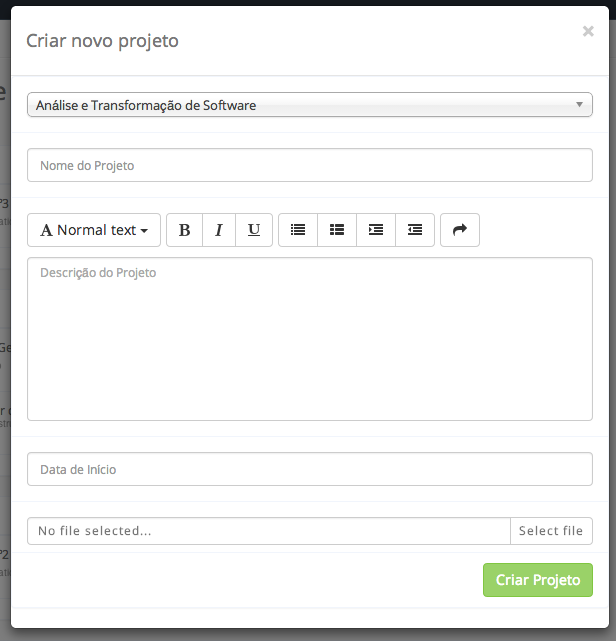
\includegraphics[width=1\textwidth,center]{images/implementacao/docentes/new_project}
  \caption{Novo projeto}
  \label{fig:teacher_project_new}
\end{figure}


Na Figura~\ref{fig:teacher_dashboard} pode ser consultada uma imagem demonstrativa da página desenvolvida.

\begin{figure}[H]
  \centering
  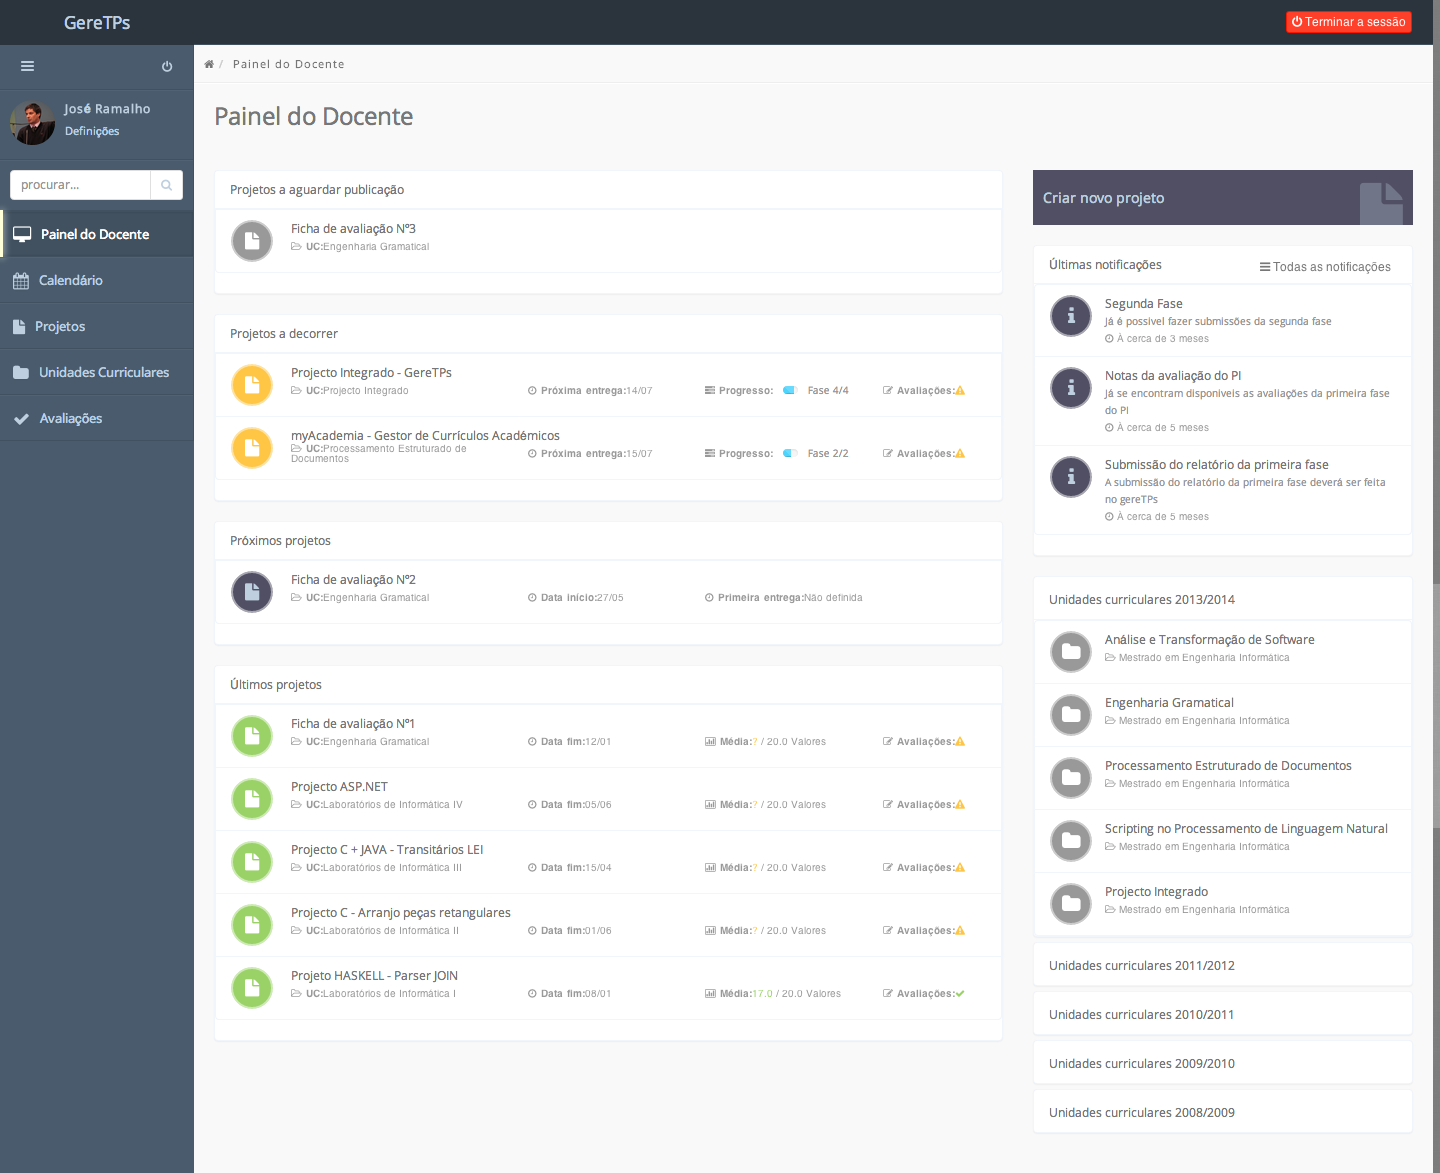
\includegraphics[width=1\textwidth,center]{images/implementacao/docentes/dashboard}
  \caption{Página inicial do painel do docente}
  \label{fig:teacher_dashboard}
\end{figure}

\subsubsection{Página de projeto}

É na página de projeto que um docente pode consultar todas as informações sobre um projeto de uma unidade curricular da qual faz parte.

Como foi descrito na secção ~\ref{ssub:student_project}, um projeto é uma das principais entidades do sistema e como tal teve-se o cuidado em garantir que o docente encontre a informação que necessita de uma forma simples e eficiente.

A diferença entre o conteúdo disponível entre a página de um projeto de um docente e de um aluno, são:

\begin{itemize}
	\item Edição de conteúdo do projeto sem necessidade de ser redirecionado para outra página
	\item Visualização e acesso as entregas efetuadas pelos alunos inscritos na unidade curricular em que o projeto de insere
	\item Ações de publicação e encerramento de um projeto
\end{itemize}

Na Figura~\ref{fig:teacher_project} pode ser consultada uma imagem demonstrativa da página desenvolvida.

\begin{figure}[H]
  \centering
  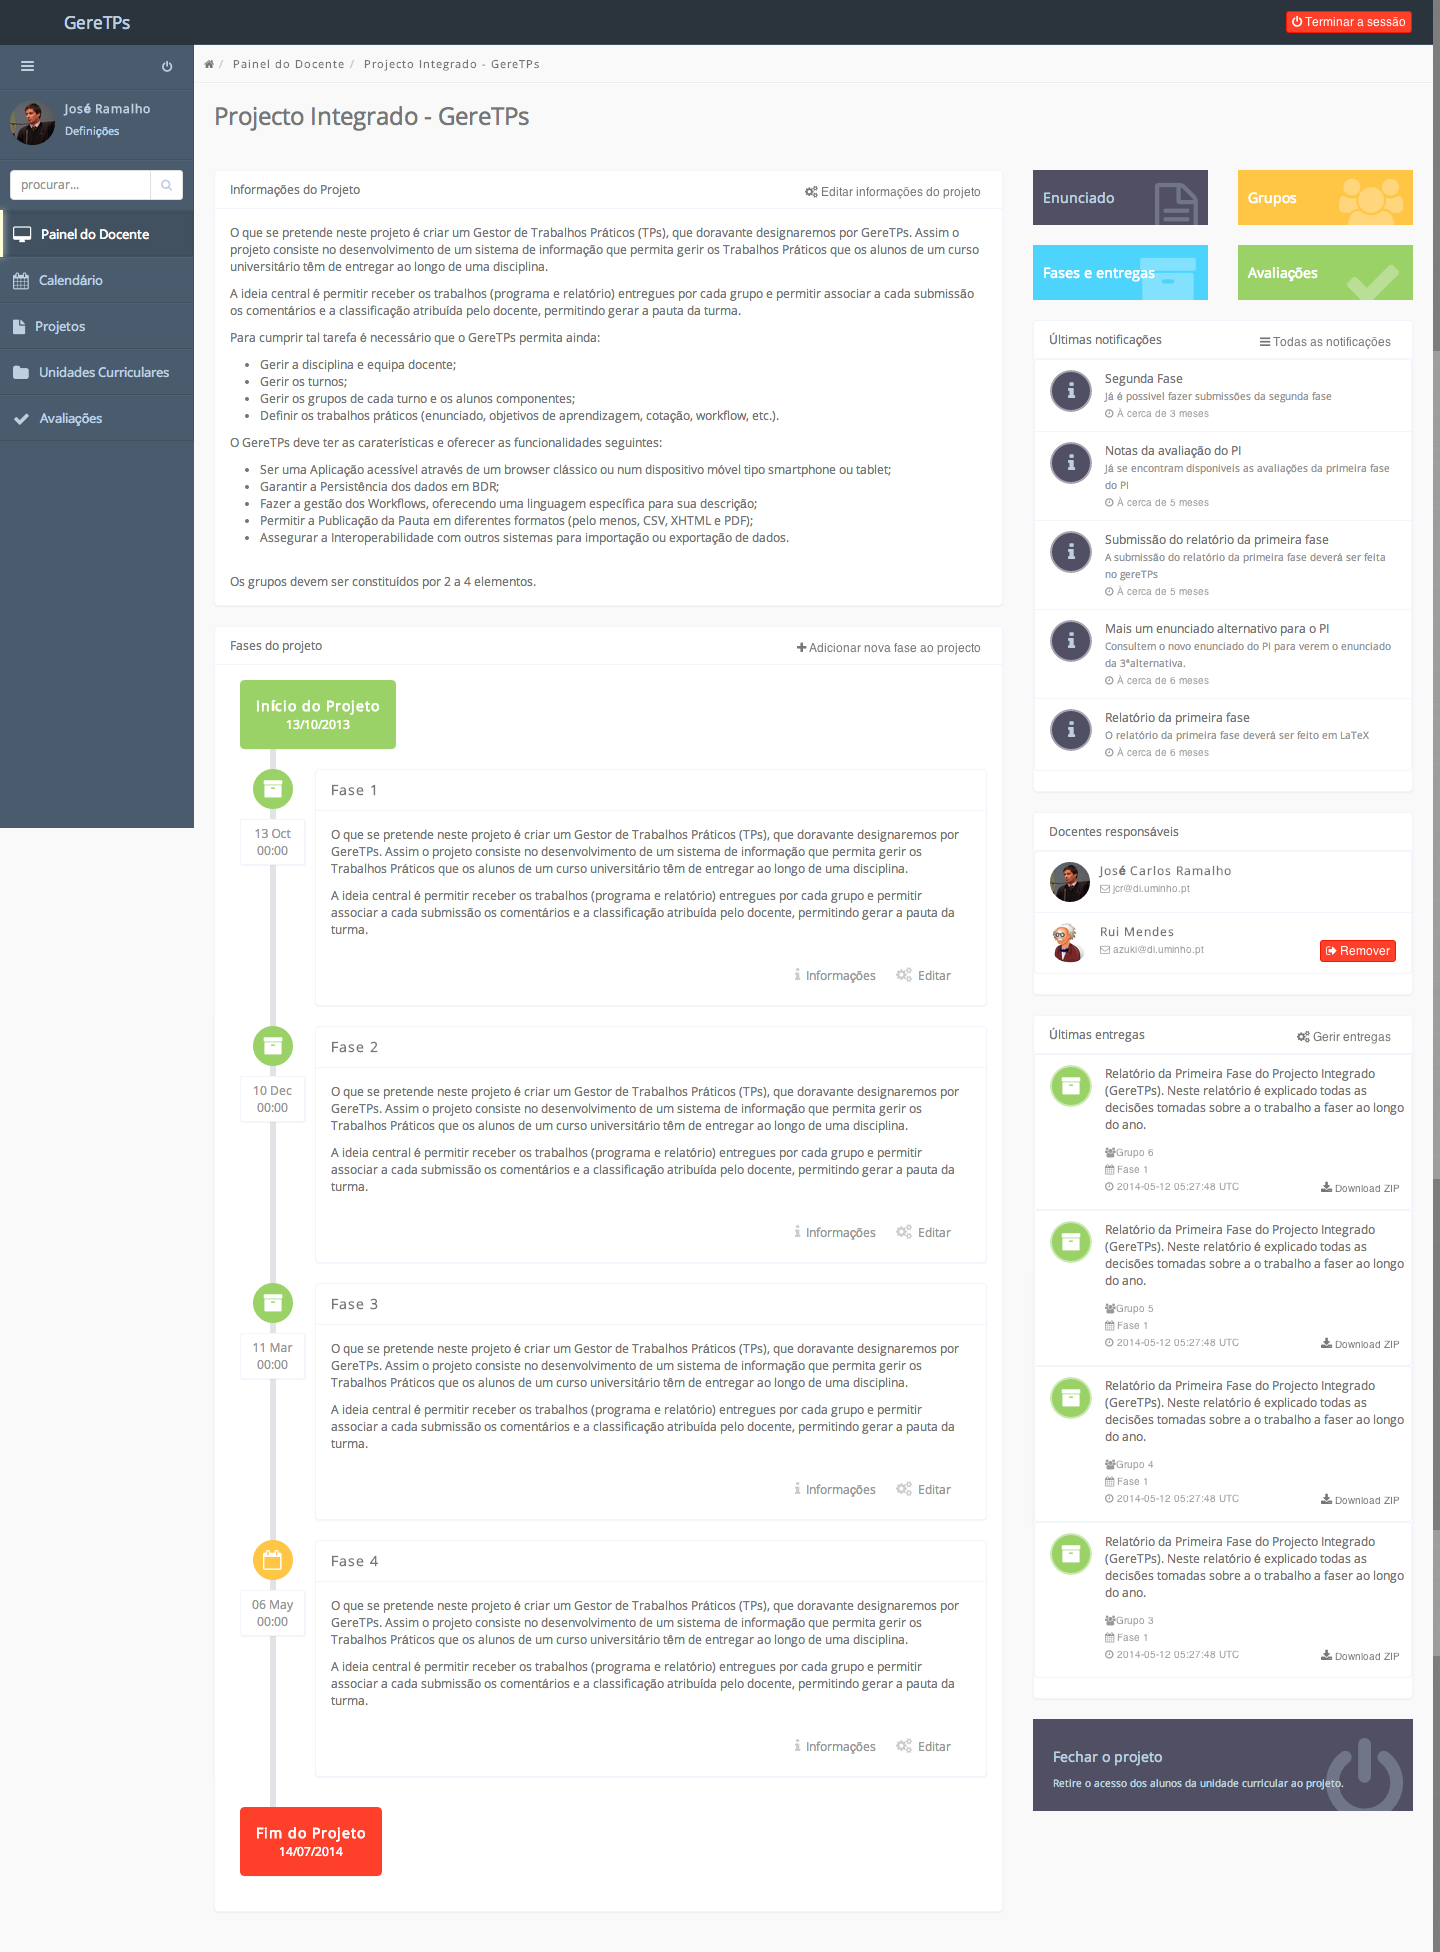
\includegraphics[width=.8\textwidth,center]{images/implementacao/docentes/project}
  \caption{Página de projeto}
  \label{fig:teacher_project}
\end{figure}

% \subsubsection{Gestão de grupos de trabalho}

\subsubsection{Gestão de fases e entregas}
\label{ssub:gestao_fases}

Na página dedicada à gestão de fases e entregas, um docente pode consultar e editar todas as informações das fases de um projeto, todas as entregas relativas às referidas fases.

Relativamente às fases, num plano principal, são apresentadas informações relativas às datas de inicio e de fim da fase, descrição, ficheiros de entrega obrigatória, ficheiros auxiliares, e atalhos para a pauta e para o enunciado da fase. Para cada fase, um docente pode consultar estatísticas, publicar a pauta e verificar quais os grupos que já efeturam entregas válidas.

Ao carregar numa entrega é possivel avaliar individualmente cada aluno. Para cada aluno, um docente pode deixar um comentário sobre a nota atribuída. Para auxiliar na da nota dada, o docente pode consultar resultados dos testes efetuados.

Na Figura~\ref{fig:teacher_deliveries} pode ser consultada uma imagem demonstrativa da página desenvolvida.

\begin{figure}[H]
  \centering
  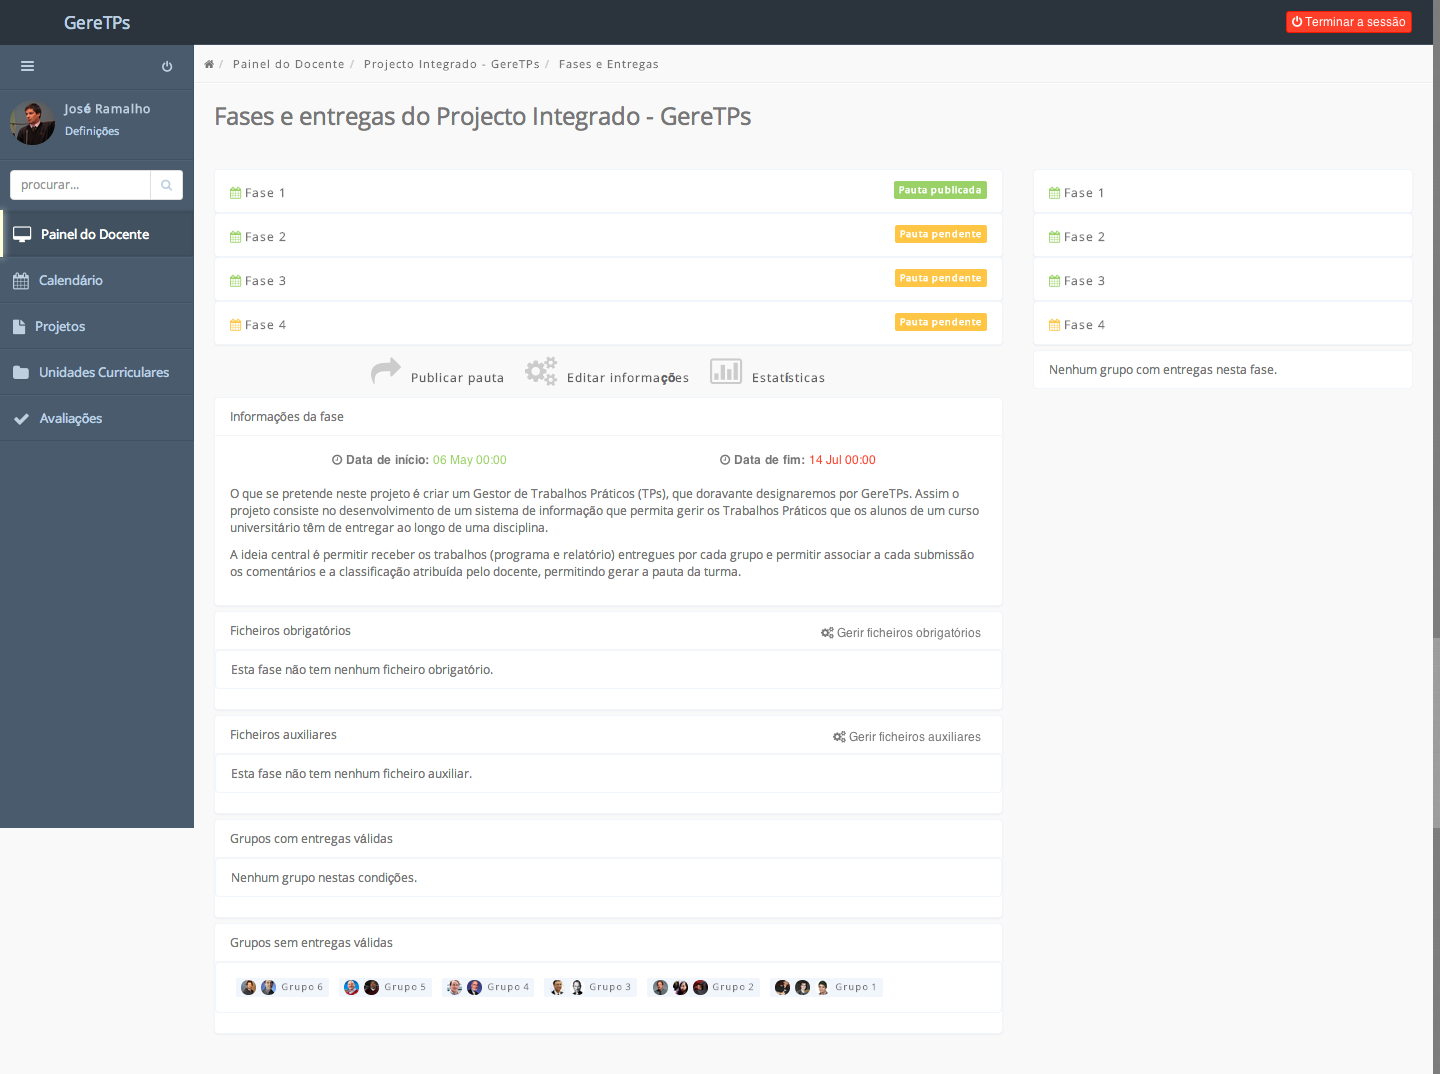
\includegraphics[width=1\textwidth,center]{images/implementacao/docentes/deliveries}
  \caption{Página de gestão de fases entregas}
  \label{fig:teacher_deliveries}
\end{figure}

% \subsubsection{Pautas de fase e projeto}

No página de gestão de um projeto, um aluno pode consultar uma pauta detalhada. Esta pauta lista todos os alunos inscritos na unidade curricular associada ao projeto e respetiva nota.

Além da nota final do projeto, também é possível ver a nota de cada fase.

Na Figura~\ref{fig:student_grades_project} pode ser consultada uma imagem demonstrativa da página desenvolvida.

\begin{figure}[H]
	\centering
	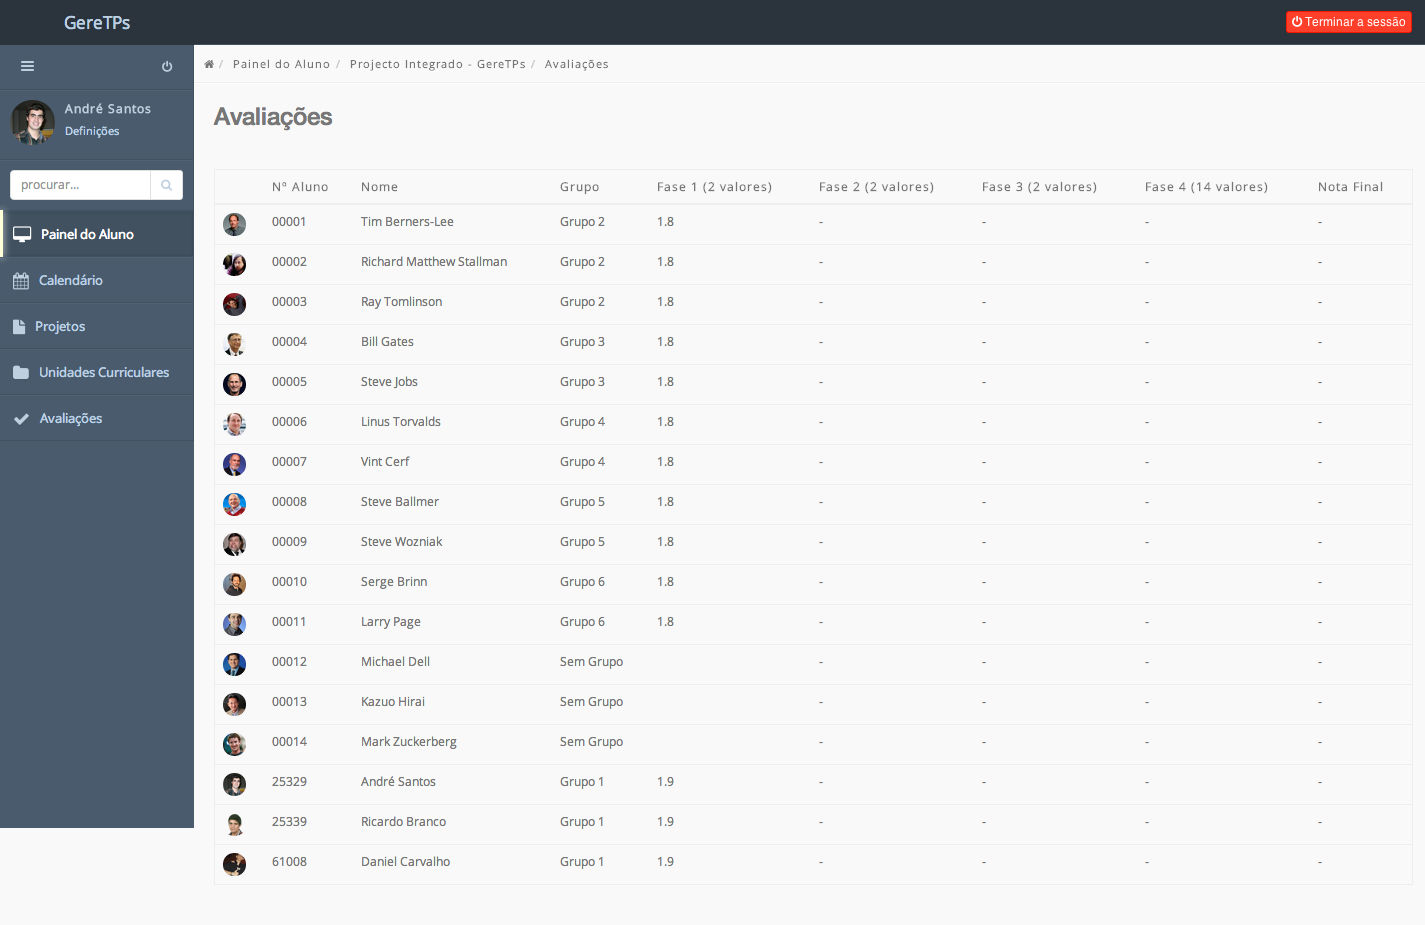
\includegraphics[width=1\textwidth,center]{images/implementacao/alunos/grades_project}
	\caption{Pauta de um projeto}
	\label{fig:student_grades_project}
\end{figure}

Ainda na página de gestão de um projeto, é possível aceder à página de \hyperref[ssub:gestao_fases]{Gestão de fases e entregas}. A partir desta página é possível um aluno consultar a pauta de uma fase de um projeto, caso esta já tenha sido lançada por um dos docentes da unidade curricular associada ao projeto.

A pauta de uma fase é bastante semelhante à pauta de um projeto, com a particularidade de esta apresentar a nota da fase entre zero e vinte valores e a nota correspondente no final do projeto.

Na Figura~\ref{fig:student_grades_phase} pode ser consultada uma imagem demonstrativa da página desenvolvida.

\begin{figure}[H]
	\centering
	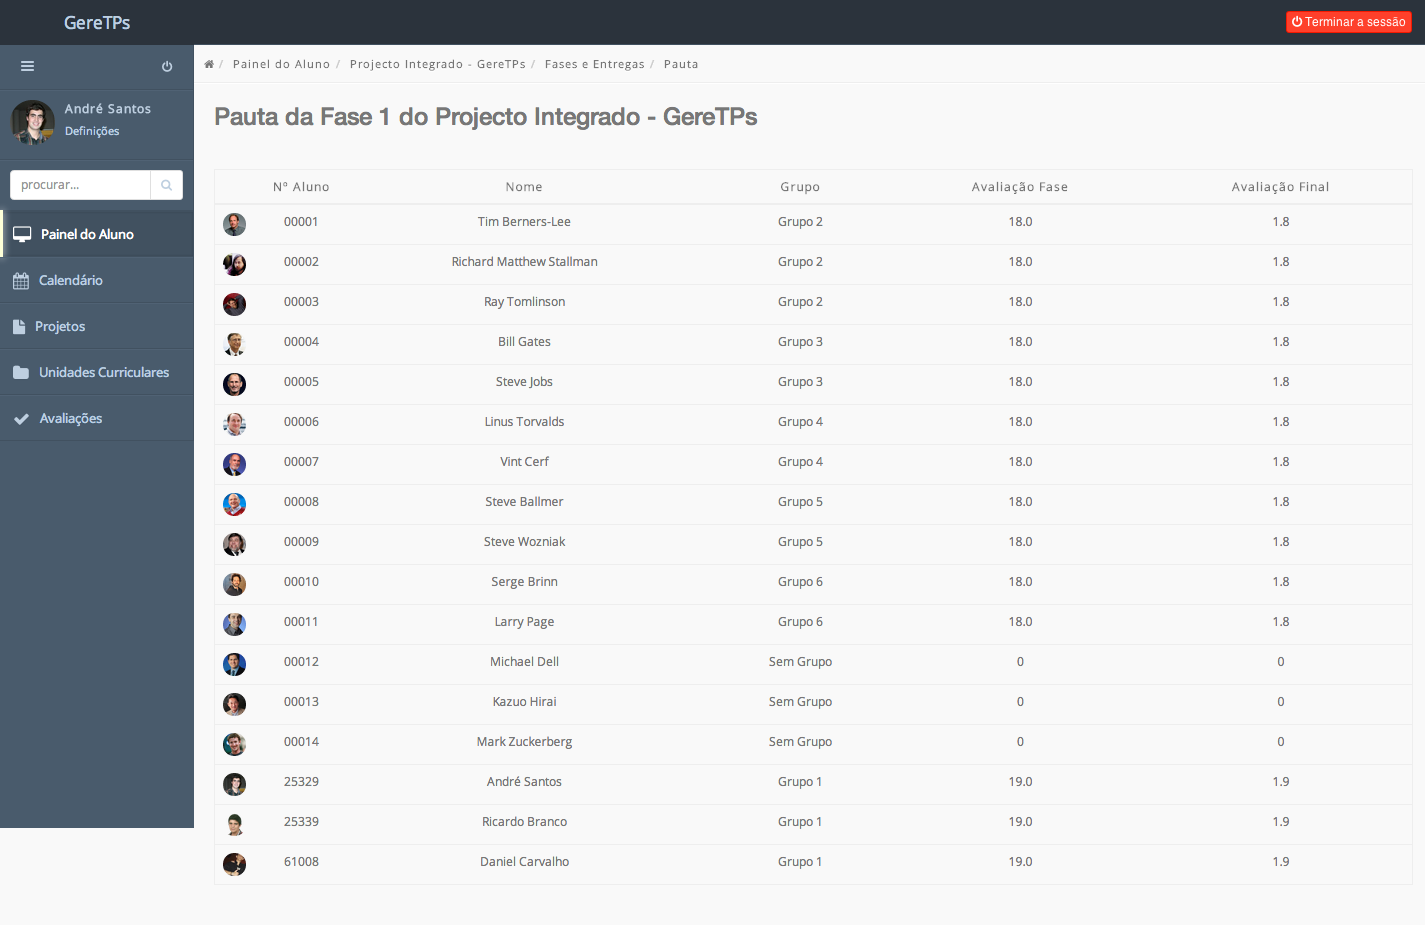
\includegraphics[width=1\textwidth,center]{images/implementacao/alunos/grades_phase}
	\caption{Pauta da uma fase}
	\label{fig:student_grades_phase}
\end{figure}

 \subsubsection{Gestão de unidades curriculares}

Na pagina de gestão de unidades curriculares, um docente pode consultar todas as unidades curriculares em que este está inserido (figura ~\ref{fig:teacher_ucs_index}) e criar uma nova unidade curricular (figura ~\ref{fig:teacher_new_uc}).


\begin{figure}[H]
  \centering
  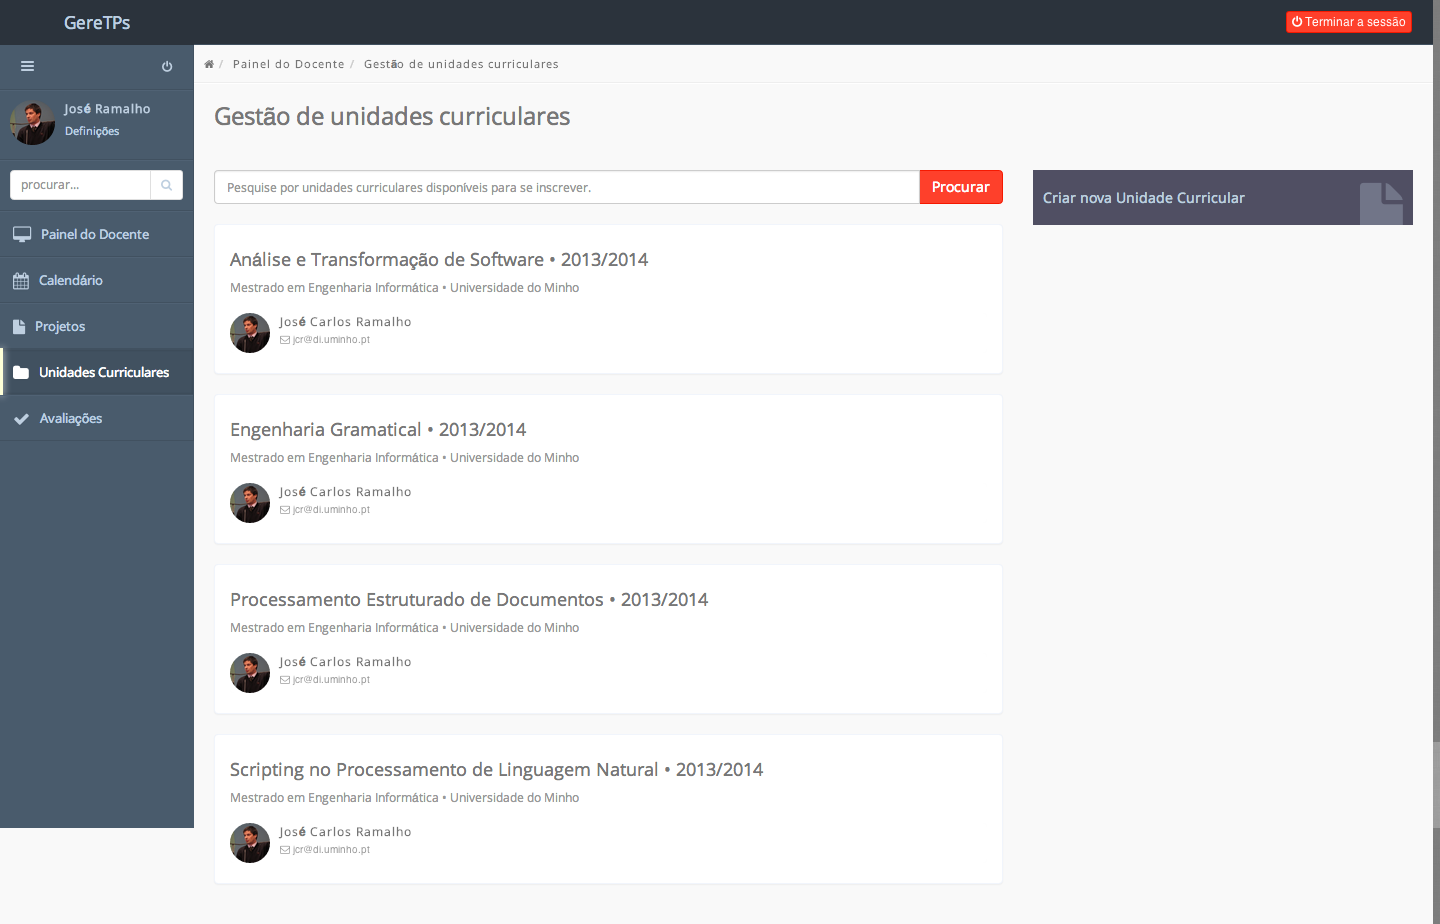
\includegraphics[width=1\textwidth,center]{images/implementacao/docentes/ucs_index}
  \caption{Página de gestão de unidades curriculares}
  \label{fig:teacher_ucs_index}
\end{figure}

\begin{figure}[H]
  \centering
  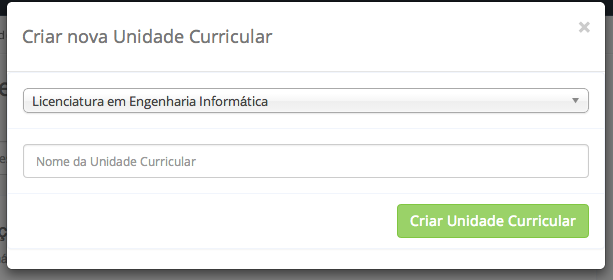
\includegraphics[width=1\textwidth,center]{images/implementacao/docentes/new_uc}
  \caption{Nova Unidade Curricular}
  \label{fig:teacher_new_uc}
\end{figure}

Após criar uma nova unidade curricular, o docente é reencaminhado para a página da unidade curricular criada.

Na página de uma unidade curricular é possível visualizar os projetos dessa unidade curricular, adicionar docentes e fazer gestão de alunos e turnos.

Na página de gestão de alunos (figura ~\ref{fig:uc_students}), um docente pode aceitar ou remover a inscrição de um aluno.

\begin{figure}[H]
  \centering
  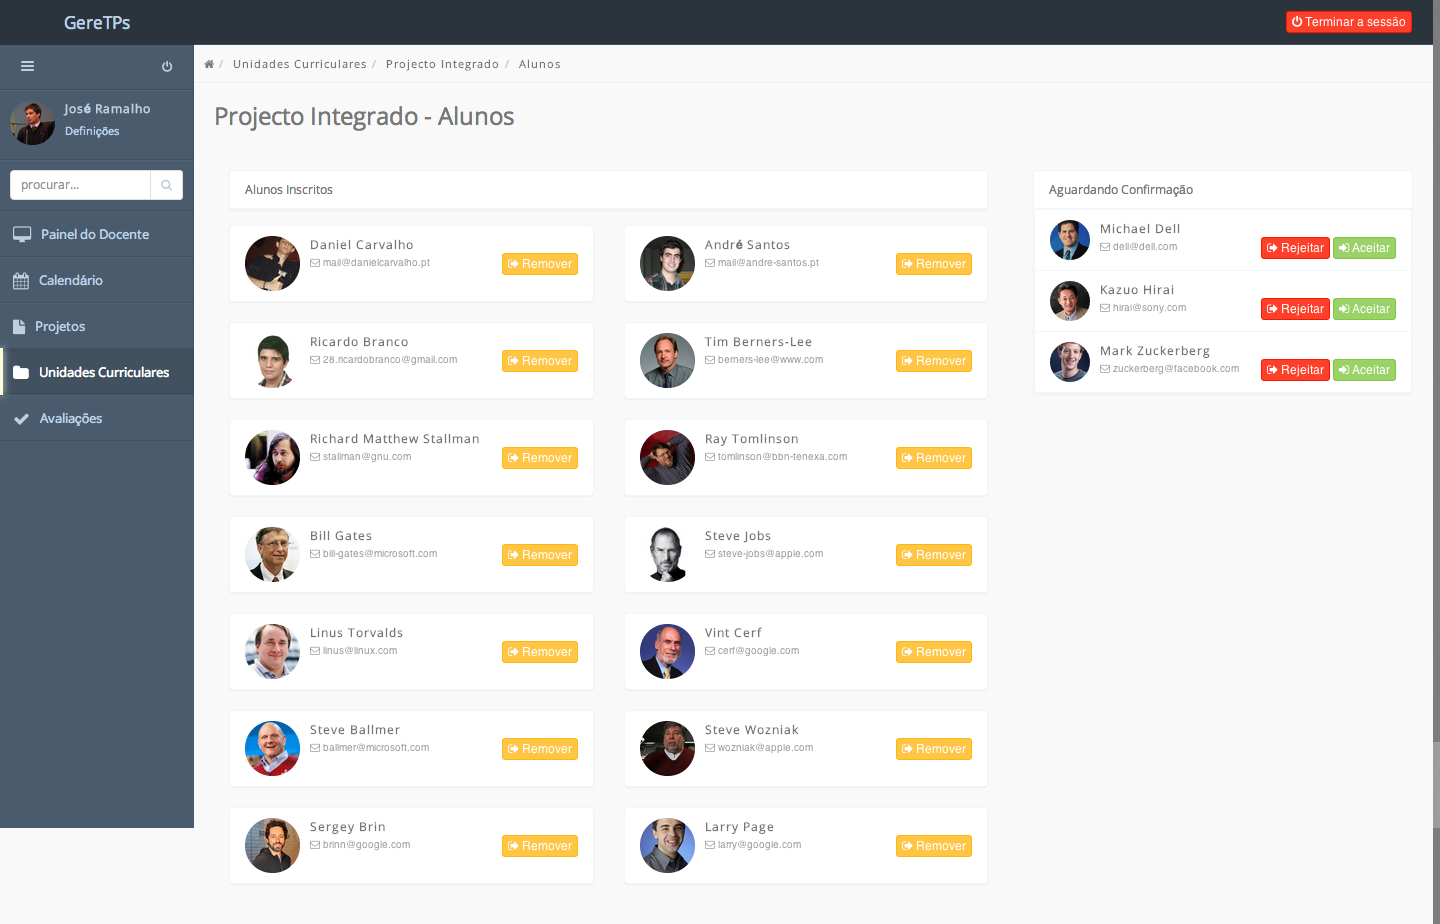
\includegraphics[width=1\textwidth,center]{images/implementacao/docentes/uc_students}
  \caption{Gestão de alunos de uma unidade curricular}
  \label{fig:uc_students}
\end{figure}


Na página de gestão de alunos (figura ~\ref{fig:uc_shifts}), um docente pode criar turnos e adicionar ou remover um aluno de um turno.

\begin{figure}[H]
  \centering
  \includegraphics[width=1\textwidth,center]{images/implementacao/docentes/uc_shifts}
  \caption{Gestão de turnos de uma unidade curricular}
  \label{fig:uc_shifts}
\end{figure}


Na Figura~\ref{fig:teacher_subjects} pode ser consultada uma imagem demonstrativa da página desenvolvida.

\begin{figure}[H]
  \centering
  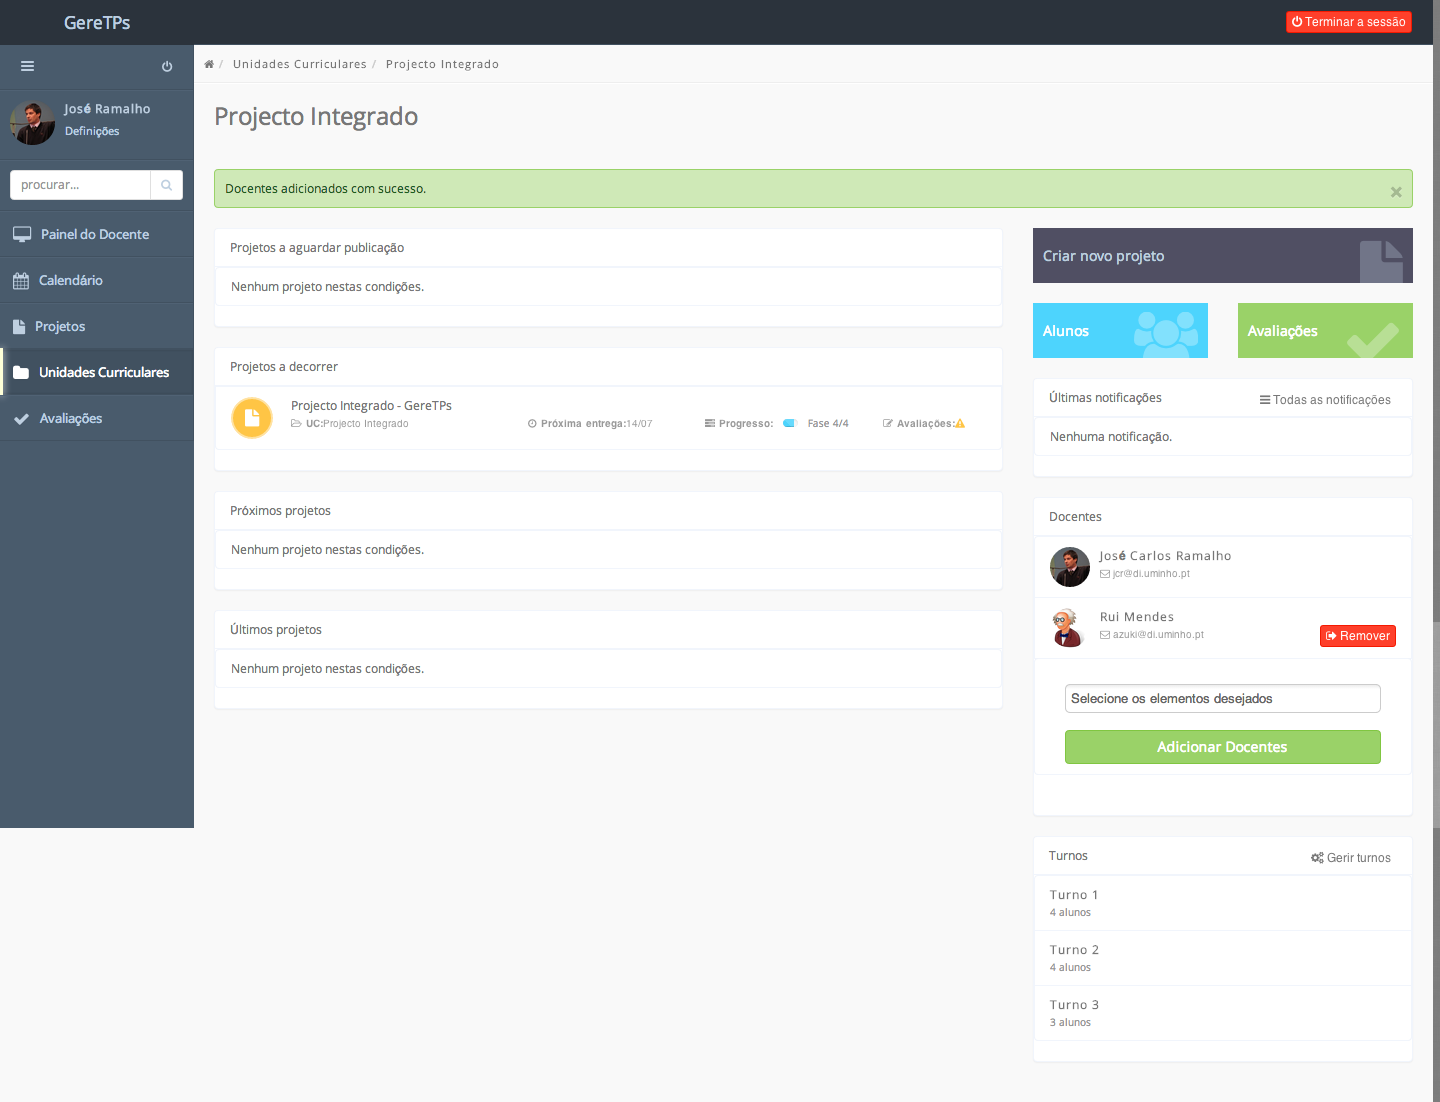
\includegraphics[width=1\textwidth,center]{images/implementacao/docentes/uc}
  \caption{Página de uma unidade curricular}
  \label{fig:teacher_subjects}
\end{figure}

 \subsubsection{Consulta e avaliação de uma entrega}
\label{ssub:entrega_avaliacao}

Ao carregar numa entrega, o utilizador é direcionado para uma página onde pode consultar as informações da referida entrega, assim como proceder à sua avaliação.\\

Nesta página o utilizador pode consultar a descrição da entrega, fazer download dos ficheiros que a constituem e consultar os resultados dos testes a que a entrega foi submetida.\\

Pode também facilmente avaliar os alunos que constituem o grupo que efetuou a entrega, indicando a sua avaliação e uma nota auxiliar.\\

Na Figura~\ref{fig:delivery_grades} pode ser consultada uma imagem demonstrativa da página desenvolvida.

\begin{figure}[H]
  \centering
  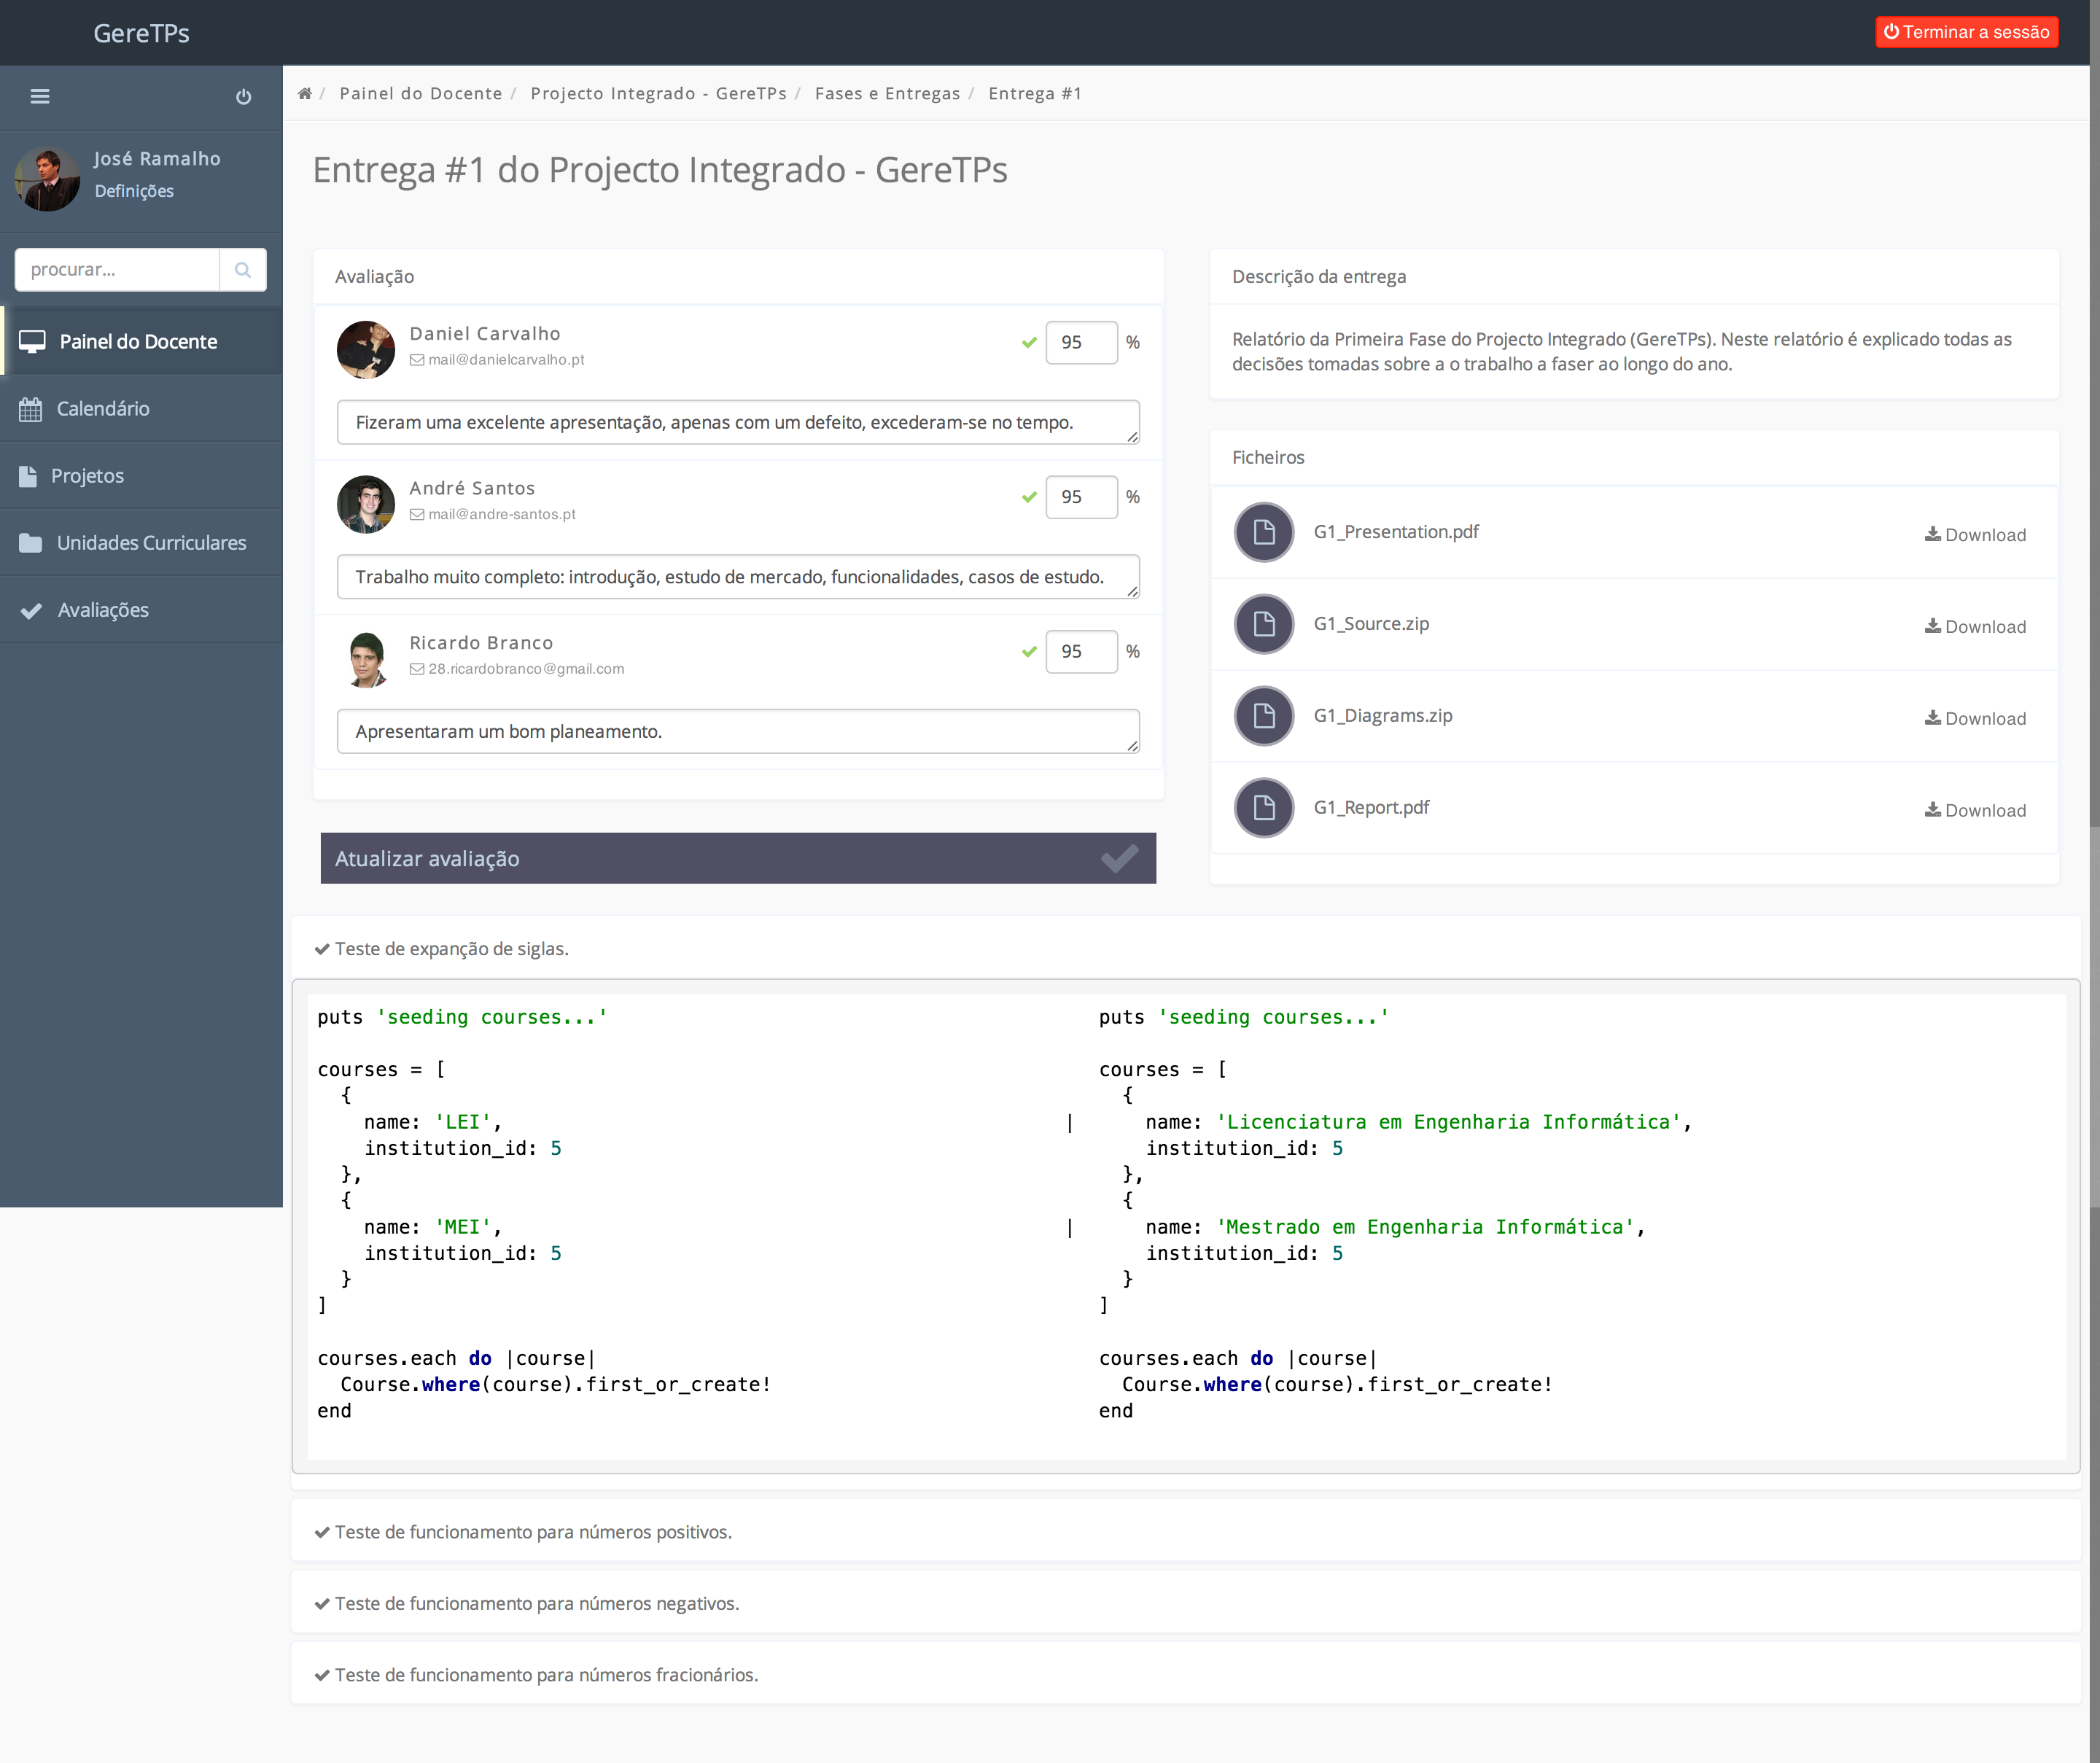
\includegraphics[width=1\textwidth,center]{images/implementacao/docentes/delivery_and_grades}
  \caption{Página de consulta e avaliação de uma entrega}
  \label{fig:delivery_grades}
\end{figure}


